% RTM truncation, after ITransverse.jl Fig. 6(b) and Fig. 9. Companion to imgs/truncation.tex.
% (a) the generalized canonical condition, imposed on the two distinct boundaries.
% (b) the derivation it enables: the singular values of the transition matrix are the square roots
%     of the eigenvalues of T^dag T; the generalized canonical form collapses every column away from
%     the cut; what survives is the pair of tensors at the cut alone.
% In every sub-diagram the bonds are drawn first and the tensors on top, so no leg crosses a shape.
%
% Standalone: compiles to imgs/rtm_truncation.pdf.
% Inline:     with \usepackage{standalone}, % RTM truncation, after ITransverse.jl Fig. 6(b) and Fig. 9. Companion to imgs/truncation.tex.
% (a) the generalized canonical condition, imposed on the two distinct boundaries.
% (b) the derivation it enables: the singular values of the transition matrix are the square roots
%     of the eigenvalues of T^dag T; the generalized canonical form collapses every column away from
%     the cut; what survives is the pair of tensors at the cut alone.
% In every sub-diagram the bonds are drawn first and the tensors on top, so no leg crosses a shape.
%
% Standalone: compiles to imgs/rtm_truncation.pdf.
% Inline:     with \usepackage{standalone}, % RTM truncation, after ITransverse.jl Fig. 6(b) and Fig. 9. Companion to imgs/truncation.tex.
% (a) the generalized canonical condition, imposed on the two distinct boundaries.
% (b) the derivation it enables: the singular values of the transition matrix are the square roots
%     of the eigenvalues of T^dag T; the generalized canonical form collapses every column away from
%     the cut; what survives is the pair of tensors at the cut alone.
% In every sub-diagram the bonds are drawn first and the tensors on top, so no leg crosses a shape.
%
% Standalone: compiles to imgs/rtm_truncation.pdf.
% Inline:     with \usepackage{standalone}, % RTM truncation, after ITransverse.jl Fig. 6(b) and Fig. 9. Companion to imgs/truncation.tex.
% (a) the generalized canonical condition, imposed on the two distinct boundaries.
% (b) the derivation it enables: the singular values of the transition matrix are the square roots
%     of the eigenvalues of T^dag T; the generalized canonical form collapses every column away from
%     the cut; what survives is the pair of tensors at the cut alone.
% In every sub-diagram the bonds are drawn first and the tensors on top, so no leg crosses a shape.
%
% Standalone: compiles to imgs/rtm_truncation.pdf.
% Inline:     with \usepackage{standalone}, \input{imgs/rtm_truncation}.
\documentclass[tikz,border=3pt]{standalone}
\usepackage{amsmath,amssymb,braket,graphicx}
\usetikzlibrary{arrows.meta,shapes.geometric}

\definecolor{tnL}{RGB}{243,116,63}
\definecolor{tnLl}{RGB}{250,190,150}
\definecolor{tnR}{RGB}{60,110,150}
\definecolor{tnRl}{RGB}{160,195,220}

\newcommand{\DX}{0.56}
\newcommand{\ST}{0.38}
\newcommand{\LO}{0.00}   % legs sit on the middle of the D, not on its flat edge
\newcommand{\HA}{0.24}   % half separation inside a pair
\newcommand{\HB}{0.72}   % outer rows of the doubled object

\newcommand{\Dhh}{0.19}   % half-height of a tensor
\newcommand{\Dbb}{0.19}   % straight body, so the D comes out as wide as it is tall

% a D-shaped tensor centred at (#1,#2), flat edge on the left, filled #3
\newcommand{\dR}[3]{%
  \filldraw[fill=#3, draw=black, line width=0.95pt]
    ({#1-(\Dbb+\Dhh)/2},{#2-\Dhh}) -- ({#1+(\Dbb-\Dhh)/2},{#2-\Dhh})
    arc[start angle=-90, end angle=90, radius=\Dhh]
    -- ({#1-(\Dbb+\Dhh)/2},{#2+\Dhh}) -- cycle;}

% grouped isometries: one wide tensor carrying the comb of physical legs it absorbed
% #1 x, #2 y, #3 fill, #4 comb direction (+1 above, -1 below)
\newcommand{\wideD}[4]{%
  \filldraw[fill=#3, draw=black, line width=0.95pt]
    (#1,{#2-\Dhh}) -- ({#1+0.50},{#2-\Dhh})
    arc[start angle=-90, end angle=90, radius=\Dhh] -- (#1,{#2+\Dhh}) -- cycle;
  \foreach \c in {0.08,0.20,0.32,0.44} {
    \draw[bond] ({#1+\c},{#2+#4*\Dhh}) -- ({#1+\c},{#2+#4*0.44});
  }}

\newcommand{\bigpar}[1]{\scalebox{1.0}[4.1]{$#1$}}
\newcommand{\hugepar}[1]{\scalebox{1.0}[6.6]{$#1$}}

\begin{document}
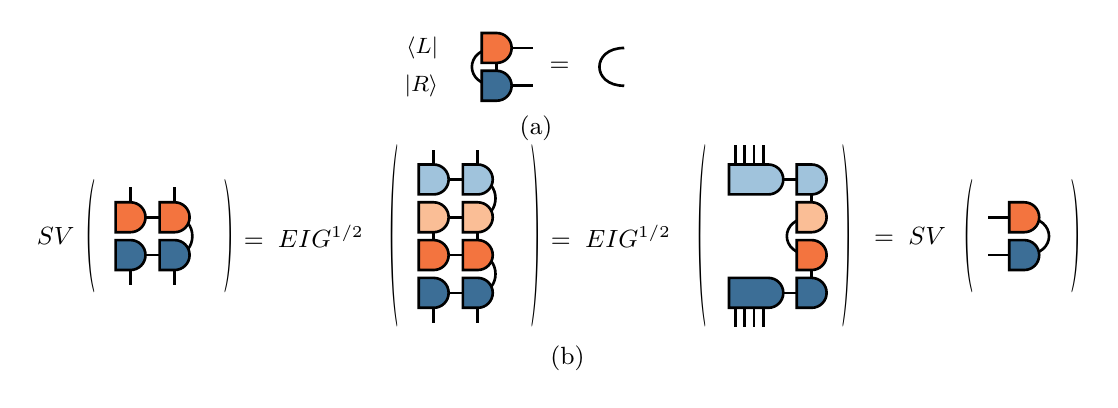
\begin{tikzpicture}[
    bond/.style={draw=black, line width=0.95pt},
    tag/.style={font=\small},
    idx/.style={font=\footnotesize},
  ]

  %% ================= (a) the generalized canonical condition =================
  \begin{scope}[xshift=5.6cm, yshift=2.15cm]
    \draw[bond] (0,\HA) .. controls (-0.42,\HA) and (-0.42,-\HA) .. (0,-\HA);
    \draw[bond] (\LO,\HA) -- (\LO,-\HA);
    \draw[bond] (0,\HA) -- (0.46,\HA);
    \draw[bond] (0,-\HA) -- (0.46,-\HA);
    \dR{0}{\HA}{tnL}
    \dR{0}{-\HA}{tnR}
    \node[idx, anchor=east] at (-0.62,\HA)  {$\bra{L}$};
    \node[idx, anchor=east] at (-0.62,-\HA) {$\ket{R}$};
    \node[tag] at (0.80,0) {$=$};
    \draw[bond] (1.62,\HA) .. controls (1.20,\HA) and (1.20,-\HA) .. (1.62,-\HA);
    \node[tag] at (0.5,-0.78) {(a)};
  \end{scope}

  %% ---- two-row chain of two sites: #1 xshift, #2 yshift, #3 top, #4 bottom, #5 open legs ----
  \newcommand{\chain}[5]{%
    \begin{scope}[xshift=#1, yshift=#2]
      \draw[bond] (0,\HA) -- (\DX,\HA);
      \draw[bond] (0,-\HA) -- (\DX,-\HA);
      \draw[bond] (\DX,\HA) .. controls ({\DX+0.30},\HA) and ({\DX+0.30},-\HA) .. (\DX,-\HA);
      \ifnum#5=1
        \foreach \i in {0,1} {
          \draw[bond] ({\i*\DX+\LO},\HA)  -- ({\i*\DX+\LO},{\HA+\ST});
          \draw[bond] ({\i*\DX+\LO},-\HA) -- ({\i*\DX+\LO},{-\HA-\ST});
        }
      \fi
      \foreach \i in {0,1} {
        \dR{\i*\DX}{\HA}{#3}
        \dR{\i*\DX}{-\HA}{#4}
      }
    \end{scope}}

  %% ================= (b): the derivation, on one line =================
  \node[tag] at (0,0) {$SV$};
  \node at (0.45,0) {\bigpar{(}};
  \chain{0.95cm}{0cm}{tnL}{tnR}{1}
  \node at (2.20,0) {\bigpar{)}};

  \node[tag] at (3.15,0) {$=\;EIG^{1/2}$};
  \node at (4.30,0) {\hugepar{(}};
  % T^dag T: the conjugate pair above the original, contracted through the middle
  \begin{scope}[xshift=4.80cm]
    \foreach \i in {0,1} {
      \draw[bond] ({\i*\DX+\LO},\HA) -- ({\i*\DX+\LO},-\HA);
      \draw[bond] ({\i*\DX+\LO},\HB) -- ({\i*\DX+\LO},{\HB+\ST});
      \draw[bond] ({\i*\DX+\LO},-\HB) -- ({\i*\DX+\LO},{-\HB-\ST});
    }
  \end{scope}
  \chain{4.80cm}{0.48cm}{tnRl}{tnLl}{0}
  \chain{4.80cm}{-0.48cm}{tnL}{tnR}{0}
  \node at (6.10,0) {\hugepar{)}};

  \node[tag] at (7.05,0) {$=\;EIG^{1/2}$};
  \node at (8.20,0) {\hugepar{(}};
  % away from the cut every column has collapsed by (a); one column survives
  \begin{scope}[xshift=8.55cm]
    \def\XC{1.05}
    \draw[bond] (0.69,\HB)  -- (\XC,\HB);
    \draw[bond] (0.69,-\HB) -- (\XC,-\HB);
    \draw[bond] ({\XC+\LO},\HB) -- ({\XC+\LO},\HA);
    \draw[bond] ({\XC+\LO},-\HA) -- ({\XC+\LO},-\HB);
    \draw[bond] (\XC,\HA) .. controls ({\XC-0.42},\HA) and ({\XC-0.42},-\HA) .. (\XC,-\HA);
    \wideD{0}{\HB}{tnRl}{1}
    \wideD{0}{-\HB}{tnR}{-1}
    \foreach \y/\f in {\HB/tnRl, \HA/tnLl, -\HA/tnL, -\HB/tnR} {
      \dR{\XC}{\y}{\f}
    }
  \end{scope}
  \node at (10.05,0) {\hugepar{)}};

  \node[tag] at (10.85,0) {$=\;SV$};
  \node at (11.60,0) {\bigpar{(}};
  \begin{scope}[xshift=12.30cm]
    \draw[bond] (0,\HA) .. controls (0.42,\HA) and (0.42,-\HA) .. (0,-\HA);
    \draw[bond] (0,\HA)  -- (-0.46,\HA);
    \draw[bond] (0,-\HA) -- (-0.46,-\HA);
    \dR{0}{\HA}{tnL}
    \dR{0}{-\HA}{tnR}
  \end{scope}
  \node at (12.95,0) {\bigpar{)}};

  \node[tag] at (6.5,-1.55) {(b)};

\end{tikzpicture}
\end{document}
.
\documentclass[tikz,border=3pt]{standalone}
\usepackage{amsmath,amssymb,braket,graphicx}
\usetikzlibrary{arrows.meta,shapes.geometric}

\definecolor{tnL}{RGB}{243,116,63}
\definecolor{tnLl}{RGB}{250,190,150}
\definecolor{tnR}{RGB}{60,110,150}
\definecolor{tnRl}{RGB}{160,195,220}

\newcommand{\DX}{0.56}
\newcommand{\ST}{0.38}
\newcommand{\LO}{0.00}   % legs sit on the middle of the D, not on its flat edge
\newcommand{\HA}{0.24}   % half separation inside a pair
\newcommand{\HB}{0.72}   % outer rows of the doubled object

\newcommand{\Dhh}{0.19}   % half-height of a tensor
\newcommand{\Dbb}{0.19}   % straight body, so the D comes out as wide as it is tall

% a D-shaped tensor centred at (#1,#2), flat edge on the left, filled #3
\newcommand{\dR}[3]{%
  \filldraw[fill=#3, draw=black, line width=0.95pt]
    ({#1-(\Dbb+\Dhh)/2},{#2-\Dhh}) -- ({#1+(\Dbb-\Dhh)/2},{#2-\Dhh})
    arc[start angle=-90, end angle=90, radius=\Dhh]
    -- ({#1-(\Dbb+\Dhh)/2},{#2+\Dhh}) -- cycle;}

% grouped isometries: one wide tensor carrying the comb of physical legs it absorbed
% #1 x, #2 y, #3 fill, #4 comb direction (+1 above, -1 below)
\newcommand{\wideD}[4]{%
  \filldraw[fill=#3, draw=black, line width=0.95pt]
    (#1,{#2-\Dhh}) -- ({#1+0.50},{#2-\Dhh})
    arc[start angle=-90, end angle=90, radius=\Dhh] -- (#1,{#2+\Dhh}) -- cycle;
  \foreach \c in {0.08,0.20,0.32,0.44} {
    \draw[bond] ({#1+\c},{#2+#4*\Dhh}) -- ({#1+\c},{#2+#4*0.44});
  }}

\newcommand{\bigpar}[1]{\scalebox{1.0}[4.1]{$#1$}}
\newcommand{\hugepar}[1]{\scalebox{1.0}[6.6]{$#1$}}

\begin{document}
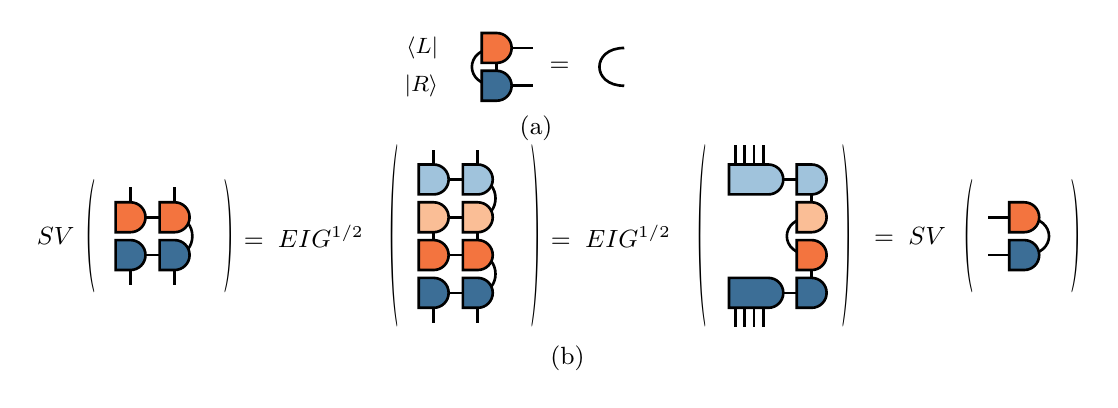
\begin{tikzpicture}[
    bond/.style={draw=black, line width=0.95pt},
    tag/.style={font=\small},
    idx/.style={font=\footnotesize},
  ]

  %% ================= (a) the generalized canonical condition =================
  \begin{scope}[xshift=5.6cm, yshift=2.15cm]
    \draw[bond] (0,\HA) .. controls (-0.42,\HA) and (-0.42,-\HA) .. (0,-\HA);
    \draw[bond] (\LO,\HA) -- (\LO,-\HA);
    \draw[bond] (0,\HA) -- (0.46,\HA);
    \draw[bond] (0,-\HA) -- (0.46,-\HA);
    \dR{0}{\HA}{tnL}
    \dR{0}{-\HA}{tnR}
    \node[idx, anchor=east] at (-0.62,\HA)  {$\bra{L}$};
    \node[idx, anchor=east] at (-0.62,-\HA) {$\ket{R}$};
    \node[tag] at (0.80,0) {$=$};
    \draw[bond] (1.62,\HA) .. controls (1.20,\HA) and (1.20,-\HA) .. (1.62,-\HA);
    \node[tag] at (0.5,-0.78) {(a)};
  \end{scope}

  %% ---- two-row chain of two sites: #1 xshift, #2 yshift, #3 top, #4 bottom, #5 open legs ----
  \newcommand{\chain}[5]{%
    \begin{scope}[xshift=#1, yshift=#2]
      \draw[bond] (0,\HA) -- (\DX,\HA);
      \draw[bond] (0,-\HA) -- (\DX,-\HA);
      \draw[bond] (\DX,\HA) .. controls ({\DX+0.30},\HA) and ({\DX+0.30},-\HA) .. (\DX,-\HA);
      \ifnum#5=1
        \foreach \i in {0,1} {
          \draw[bond] ({\i*\DX+\LO},\HA)  -- ({\i*\DX+\LO},{\HA+\ST});
          \draw[bond] ({\i*\DX+\LO},-\HA) -- ({\i*\DX+\LO},{-\HA-\ST});
        }
      \fi
      \foreach \i in {0,1} {
        \dR{\i*\DX}{\HA}{#3}
        \dR{\i*\DX}{-\HA}{#4}
      }
    \end{scope}}

  %% ================= (b): the derivation, on one line =================
  \node[tag] at (0,0) {$SV$};
  \node at (0.45,0) {\bigpar{(}};
  \chain{0.95cm}{0cm}{tnL}{tnR}{1}
  \node at (2.20,0) {\bigpar{)}};

  \node[tag] at (3.15,0) {$=\;EIG^{1/2}$};
  \node at (4.30,0) {\hugepar{(}};
  % T^dag T: the conjugate pair above the original, contracted through the middle
  \begin{scope}[xshift=4.80cm]
    \foreach \i in {0,1} {
      \draw[bond] ({\i*\DX+\LO},\HA) -- ({\i*\DX+\LO},-\HA);
      \draw[bond] ({\i*\DX+\LO},\HB) -- ({\i*\DX+\LO},{\HB+\ST});
      \draw[bond] ({\i*\DX+\LO},-\HB) -- ({\i*\DX+\LO},{-\HB-\ST});
    }
  \end{scope}
  \chain{4.80cm}{0.48cm}{tnRl}{tnLl}{0}
  \chain{4.80cm}{-0.48cm}{tnL}{tnR}{0}
  \node at (6.10,0) {\hugepar{)}};

  \node[tag] at (7.05,0) {$=\;EIG^{1/2}$};
  \node at (8.20,0) {\hugepar{(}};
  % away from the cut every column has collapsed by (a); one column survives
  \begin{scope}[xshift=8.55cm]
    \def\XC{1.05}
    \draw[bond] (0.69,\HB)  -- (\XC,\HB);
    \draw[bond] (0.69,-\HB) -- (\XC,-\HB);
    \draw[bond] ({\XC+\LO},\HB) -- ({\XC+\LO},\HA);
    \draw[bond] ({\XC+\LO},-\HA) -- ({\XC+\LO},-\HB);
    \draw[bond] (\XC,\HA) .. controls ({\XC-0.42},\HA) and ({\XC-0.42},-\HA) .. (\XC,-\HA);
    \wideD{0}{\HB}{tnRl}{1}
    \wideD{0}{-\HB}{tnR}{-1}
    \foreach \y/\f in {\HB/tnRl, \HA/tnLl, -\HA/tnL, -\HB/tnR} {
      \dR{\XC}{\y}{\f}
    }
  \end{scope}
  \node at (10.05,0) {\hugepar{)}};

  \node[tag] at (10.85,0) {$=\;SV$};
  \node at (11.60,0) {\bigpar{(}};
  \begin{scope}[xshift=12.30cm]
    \draw[bond] (0,\HA) .. controls (0.42,\HA) and (0.42,-\HA) .. (0,-\HA);
    \draw[bond] (0,\HA)  -- (-0.46,\HA);
    \draw[bond] (0,-\HA) -- (-0.46,-\HA);
    \dR{0}{\HA}{tnL}
    \dR{0}{-\HA}{tnR}
  \end{scope}
  \node at (12.95,0) {\bigpar{)}};

  \node[tag] at (6.5,-1.55) {(b)};

\end{tikzpicture}
\end{document}
.
\documentclass[tikz,border=3pt]{standalone}
\usepackage{amsmath,amssymb,braket,graphicx}
\usetikzlibrary{arrows.meta,shapes.geometric}

\definecolor{tnL}{RGB}{243,116,63}
\definecolor{tnLl}{RGB}{250,190,150}
\definecolor{tnR}{RGB}{60,110,150}
\definecolor{tnRl}{RGB}{160,195,220}

\newcommand{\DX}{0.56}
\newcommand{\ST}{0.38}
\newcommand{\LO}{0.00}   % legs sit on the middle of the D, not on its flat edge
\newcommand{\HA}{0.24}   % half separation inside a pair
\newcommand{\HB}{0.72}   % outer rows of the doubled object

\newcommand{\Dhh}{0.19}   % half-height of a tensor
\newcommand{\Dbb}{0.19}   % straight body, so the D comes out as wide as it is tall

% a D-shaped tensor centred at (#1,#2), flat edge on the left, filled #3
\newcommand{\dR}[3]{%
  \filldraw[fill=#3, draw=black, line width=0.95pt]
    ({#1-(\Dbb+\Dhh)/2},{#2-\Dhh}) -- ({#1+(\Dbb-\Dhh)/2},{#2-\Dhh})
    arc[start angle=-90, end angle=90, radius=\Dhh]
    -- ({#1-(\Dbb+\Dhh)/2},{#2+\Dhh}) -- cycle;}

% grouped isometries: one wide tensor carrying the comb of physical legs it absorbed
% #1 x, #2 y, #3 fill, #4 comb direction (+1 above, -1 below)
\newcommand{\wideD}[4]{%
  \filldraw[fill=#3, draw=black, line width=0.95pt]
    (#1,{#2-\Dhh}) -- ({#1+0.50},{#2-\Dhh})
    arc[start angle=-90, end angle=90, radius=\Dhh] -- (#1,{#2+\Dhh}) -- cycle;
  \foreach \c in {0.08,0.20,0.32,0.44} {
    \draw[bond] ({#1+\c},{#2+#4*\Dhh}) -- ({#1+\c},{#2+#4*0.44});
  }}

\newcommand{\bigpar}[1]{\scalebox{1.0}[4.1]{$#1$}}
\newcommand{\hugepar}[1]{\scalebox{1.0}[6.6]{$#1$}}

\begin{document}
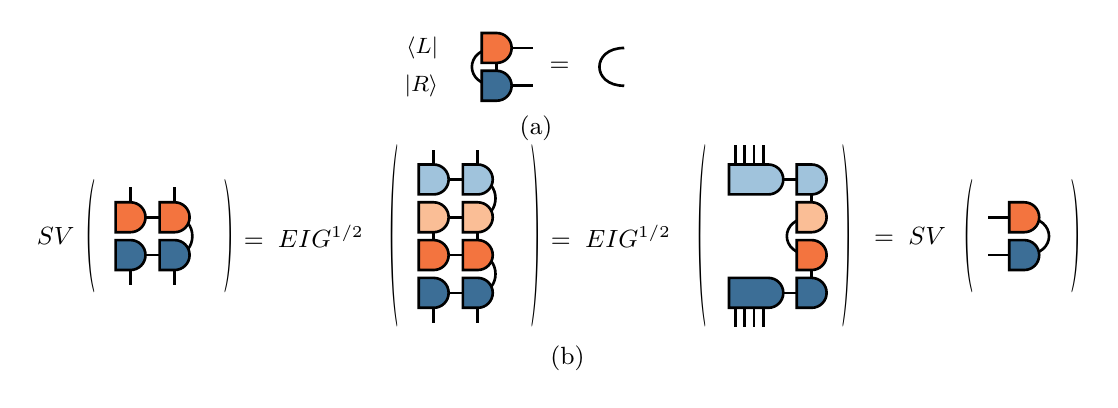
\begin{tikzpicture}[
    bond/.style={draw=black, line width=0.95pt},
    tag/.style={font=\small},
    idx/.style={font=\footnotesize},
  ]

  %% ================= (a) the generalized canonical condition =================
  \begin{scope}[xshift=5.6cm, yshift=2.15cm]
    \draw[bond] (0,\HA) .. controls (-0.42,\HA) and (-0.42,-\HA) .. (0,-\HA);
    \draw[bond] (\LO,\HA) -- (\LO,-\HA);
    \draw[bond] (0,\HA) -- (0.46,\HA);
    \draw[bond] (0,-\HA) -- (0.46,-\HA);
    \dR{0}{\HA}{tnL}
    \dR{0}{-\HA}{tnR}
    \node[idx, anchor=east] at (-0.62,\HA)  {$\bra{L}$};
    \node[idx, anchor=east] at (-0.62,-\HA) {$\ket{R}$};
    \node[tag] at (0.80,0) {$=$};
    \draw[bond] (1.62,\HA) .. controls (1.20,\HA) and (1.20,-\HA) .. (1.62,-\HA);
    \node[tag] at (0.5,-0.78) {(a)};
  \end{scope}

  %% ---- two-row chain of two sites: #1 xshift, #2 yshift, #3 top, #4 bottom, #5 open legs ----
  \newcommand{\chain}[5]{%
    \begin{scope}[xshift=#1, yshift=#2]
      \draw[bond] (0,\HA) -- (\DX,\HA);
      \draw[bond] (0,-\HA) -- (\DX,-\HA);
      \draw[bond] (\DX,\HA) .. controls ({\DX+0.30},\HA) and ({\DX+0.30},-\HA) .. (\DX,-\HA);
      \ifnum#5=1
        \foreach \i in {0,1} {
          \draw[bond] ({\i*\DX+\LO},\HA)  -- ({\i*\DX+\LO},{\HA+\ST});
          \draw[bond] ({\i*\DX+\LO},-\HA) -- ({\i*\DX+\LO},{-\HA-\ST});
        }
      \fi
      \foreach \i in {0,1} {
        \dR{\i*\DX}{\HA}{#3}
        \dR{\i*\DX}{-\HA}{#4}
      }
    \end{scope}}

  %% ================= (b): the derivation, on one line =================
  \node[tag] at (0,0) {$SV$};
  \node at (0.45,0) {\bigpar{(}};
  \chain{0.95cm}{0cm}{tnL}{tnR}{1}
  \node at (2.20,0) {\bigpar{)}};

  \node[tag] at (3.15,0) {$=\;EIG^{1/2}$};
  \node at (4.30,0) {\hugepar{(}};
  % T^dag T: the conjugate pair above the original, contracted through the middle
  \begin{scope}[xshift=4.80cm]
    \foreach \i in {0,1} {
      \draw[bond] ({\i*\DX+\LO},\HA) -- ({\i*\DX+\LO},-\HA);
      \draw[bond] ({\i*\DX+\LO},\HB) -- ({\i*\DX+\LO},{\HB+\ST});
      \draw[bond] ({\i*\DX+\LO},-\HB) -- ({\i*\DX+\LO},{-\HB-\ST});
    }
  \end{scope}
  \chain{4.80cm}{0.48cm}{tnRl}{tnLl}{0}
  \chain{4.80cm}{-0.48cm}{tnL}{tnR}{0}
  \node at (6.10,0) {\hugepar{)}};

  \node[tag] at (7.05,0) {$=\;EIG^{1/2}$};
  \node at (8.20,0) {\hugepar{(}};
  % away from the cut every column has collapsed by (a); one column survives
  \begin{scope}[xshift=8.55cm]
    \def\XC{1.05}
    \draw[bond] (0.69,\HB)  -- (\XC,\HB);
    \draw[bond] (0.69,-\HB) -- (\XC,-\HB);
    \draw[bond] ({\XC+\LO},\HB) -- ({\XC+\LO},\HA);
    \draw[bond] ({\XC+\LO},-\HA) -- ({\XC+\LO},-\HB);
    \draw[bond] (\XC,\HA) .. controls ({\XC-0.42},\HA) and ({\XC-0.42},-\HA) .. (\XC,-\HA);
    \wideD{0}{\HB}{tnRl}{1}
    \wideD{0}{-\HB}{tnR}{-1}
    \foreach \y/\f in {\HB/tnRl, \HA/tnLl, -\HA/tnL, -\HB/tnR} {
      \dR{\XC}{\y}{\f}
    }
  \end{scope}
  \node at (10.05,0) {\hugepar{)}};

  \node[tag] at (10.85,0) {$=\;SV$};
  \node at (11.60,0) {\bigpar{(}};
  \begin{scope}[xshift=12.30cm]
    \draw[bond] (0,\HA) .. controls (0.42,\HA) and (0.42,-\HA) .. (0,-\HA);
    \draw[bond] (0,\HA)  -- (-0.46,\HA);
    \draw[bond] (0,-\HA) -- (-0.46,-\HA);
    \dR{0}{\HA}{tnL}
    \dR{0}{-\HA}{tnR}
  \end{scope}
  \node at (12.95,0) {\bigpar{)}};

  \node[tag] at (6.5,-1.55) {(b)};

\end{tikzpicture}
\end{document}
.
\documentclass[tikz,border=3pt]{standalone}
\usepackage{amsmath,amssymb,braket,graphicx}
\usetikzlibrary{arrows.meta,shapes.geometric}

\definecolor{tnL}{RGB}{243,116,63}
\definecolor{tnLl}{RGB}{250,190,150}
\definecolor{tnR}{RGB}{60,110,150}
\definecolor{tnRl}{RGB}{160,195,220}

\newcommand{\DX}{0.56}
\newcommand{\ST}{0.38}
\newcommand{\LO}{0.00}   % legs sit on the middle of the D, not on its flat edge
\newcommand{\HA}{0.24}   % half separation inside a pair
\newcommand{\HB}{0.72}   % outer rows of the doubled object

\newcommand{\Dhh}{0.19}   % half-height of a tensor
\newcommand{\Dbb}{0.19}   % straight body, so the D comes out as wide as it is tall

% a D-shaped tensor centred at (#1,#2), flat edge on the left, filled #3
\newcommand{\dR}[3]{%
  \filldraw[fill=#3, draw=black, line width=0.95pt]
    ({#1-(\Dbb+\Dhh)/2},{#2-\Dhh}) -- ({#1+(\Dbb-\Dhh)/2},{#2-\Dhh})
    arc[start angle=-90, end angle=90, radius=\Dhh]
    -- ({#1-(\Dbb+\Dhh)/2},{#2+\Dhh}) -- cycle;}

% grouped isometries: one wide tensor carrying the comb of physical legs it absorbed
% #1 x, #2 y, #3 fill, #4 comb direction (+1 above, -1 below)
\newcommand{\wideD}[4]{%
  \filldraw[fill=#3, draw=black, line width=0.95pt]
    (#1,{#2-\Dhh}) -- ({#1+0.50},{#2-\Dhh})
    arc[start angle=-90, end angle=90, radius=\Dhh] -- (#1,{#2+\Dhh}) -- cycle;
  \foreach \c in {0.08,0.20,0.32,0.44} {
    \draw[bond] ({#1+\c},{#2+#4*\Dhh}) -- ({#1+\c},{#2+#4*0.44});
  }}

\newcommand{\bigpar}[1]{\scalebox{1.0}[4.1]{$#1$}}
\newcommand{\hugepar}[1]{\scalebox{1.0}[6.6]{$#1$}}

\begin{document}
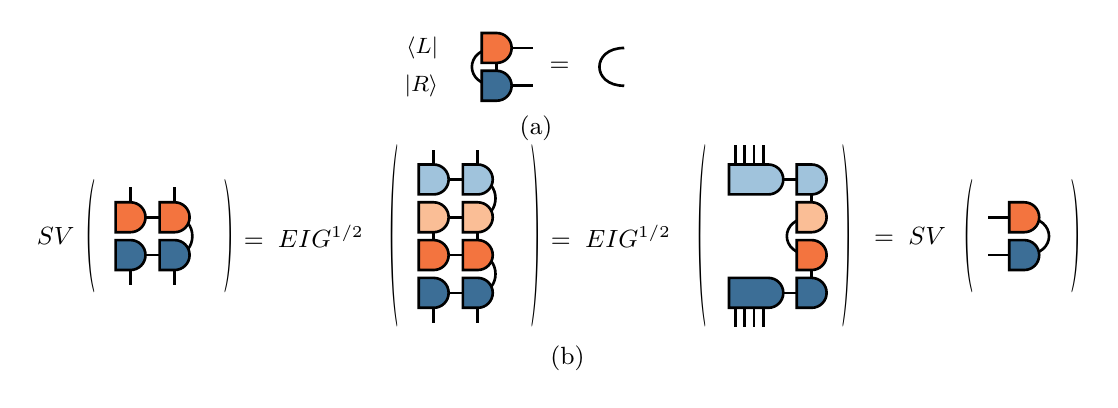
\begin{tikzpicture}[
    bond/.style={draw=black, line width=0.95pt},
    tag/.style={font=\small},
    idx/.style={font=\footnotesize},
  ]

  %% ================= (a) the generalized canonical condition =================
  \begin{scope}[xshift=5.6cm, yshift=2.15cm]
    \draw[bond] (0,\HA) .. controls (-0.42,\HA) and (-0.42,-\HA) .. (0,-\HA);
    \draw[bond] (\LO,\HA) -- (\LO,-\HA);
    \draw[bond] (0,\HA) -- (0.46,\HA);
    \draw[bond] (0,-\HA) -- (0.46,-\HA);
    \dR{0}{\HA}{tnL}
    \dR{0}{-\HA}{tnR}
    \node[idx, anchor=east] at (-0.62,\HA)  {$\bra{L}$};
    \node[idx, anchor=east] at (-0.62,-\HA) {$\ket{R}$};
    \node[tag] at (0.80,0) {$=$};
    \draw[bond] (1.62,\HA) .. controls (1.20,\HA) and (1.20,-\HA) .. (1.62,-\HA);
    \node[tag] at (0.5,-0.78) {(a)};
  \end{scope}

  %% ---- two-row chain of two sites: #1 xshift, #2 yshift, #3 top, #4 bottom, #5 open legs ----
  \newcommand{\chain}[5]{%
    \begin{scope}[xshift=#1, yshift=#2]
      \draw[bond] (0,\HA) -- (\DX,\HA);
      \draw[bond] (0,-\HA) -- (\DX,-\HA);
      \draw[bond] (\DX,\HA) .. controls ({\DX+0.30},\HA) and ({\DX+0.30},-\HA) .. (\DX,-\HA);
      \ifnum#5=1
        \foreach \i in {0,1} {
          \draw[bond] ({\i*\DX+\LO},\HA)  -- ({\i*\DX+\LO},{\HA+\ST});
          \draw[bond] ({\i*\DX+\LO},-\HA) -- ({\i*\DX+\LO},{-\HA-\ST});
        }
      \fi
      \foreach \i in {0,1} {
        \dR{\i*\DX}{\HA}{#3}
        \dR{\i*\DX}{-\HA}{#4}
      }
    \end{scope}}

  %% ================= (b): the derivation, on one line =================
  \node[tag] at (0,0) {$SV$};
  \node at (0.45,0) {\bigpar{(}};
  \chain{0.95cm}{0cm}{tnL}{tnR}{1}
  \node at (2.20,0) {\bigpar{)}};

  \node[tag] at (3.15,0) {$=\;EIG^{1/2}$};
  \node at (4.30,0) {\hugepar{(}};
  % T^dag T: the conjugate pair above the original, contracted through the middle
  \begin{scope}[xshift=4.80cm]
    \foreach \i in {0,1} {
      \draw[bond] ({\i*\DX+\LO},\HA) -- ({\i*\DX+\LO},-\HA);
      \draw[bond] ({\i*\DX+\LO},\HB) -- ({\i*\DX+\LO},{\HB+\ST});
      \draw[bond] ({\i*\DX+\LO},-\HB) -- ({\i*\DX+\LO},{-\HB-\ST});
    }
  \end{scope}
  \chain{4.80cm}{0.48cm}{tnRl}{tnLl}{0}
  \chain{4.80cm}{-0.48cm}{tnL}{tnR}{0}
  \node at (6.10,0) {\hugepar{)}};

  \node[tag] at (7.05,0) {$=\;EIG^{1/2}$};
  \node at (8.20,0) {\hugepar{(}};
  % away from the cut every column has collapsed by (a); one column survives
  \begin{scope}[xshift=8.55cm]
    \def\XC{1.05}
    \draw[bond] (0.69,\HB)  -- (\XC,\HB);
    \draw[bond] (0.69,-\HB) -- (\XC,-\HB);
    \draw[bond] ({\XC+\LO},\HB) -- ({\XC+\LO},\HA);
    \draw[bond] ({\XC+\LO},-\HA) -- ({\XC+\LO},-\HB);
    \draw[bond] (\XC,\HA) .. controls ({\XC-0.42},\HA) and ({\XC-0.42},-\HA) .. (\XC,-\HA);
    \wideD{0}{\HB}{tnRl}{1}
    \wideD{0}{-\HB}{tnR}{-1}
    \foreach \y/\f in {\HB/tnRl, \HA/tnLl, -\HA/tnL, -\HB/tnR} {
      \dR{\XC}{\y}{\f}
    }
  \end{scope}
  \node at (10.05,0) {\hugepar{)}};

  \node[tag] at (10.85,0) {$=\;SV$};
  \node at (11.60,0) {\bigpar{(}};
  \begin{scope}[xshift=12.30cm]
    \draw[bond] (0,\HA) .. controls (0.42,\HA) and (0.42,-\HA) .. (0,-\HA);
    \draw[bond] (0,\HA)  -- (-0.46,\HA);
    \draw[bond] (0,-\HA) -- (-0.46,-\HA);
    \dR{0}{\HA}{tnL}
    \dR{0}{-\HA}{tnR}
  \end{scope}
  \node at (12.95,0) {\bigpar{)}};

  \node[tag] at (6.5,-1.55) {(b)};

\end{tikzpicture}
\end{document}
